% -*- TeX -*- -*- UK -*- -*- BMR -*-
% ----------------------------------------------------------------
% Beamer presentation ************************************************
%
% Subhaneil Lahiri's template
%
% To compile:
%   Ctrl-Shift-P
%
% **** -----------------------------------------------------------
\documentclass{beamer}%[hyperref={backref=slide}]

%\input{sl_slide_preamble.tex}
\input{sl_slide_preamble_nonotes.tex}
\input{sl_slide_graphics_preamble.tex}
\input{sl_definitions.tex}
\input{sl_slide_symbols.tex}
%
\usecolortheme[rgb={0.37843137 0.07058824 0.5372549}]{structure}
%
\graphicspath{{"Figures/"}}
%matrices
\newcommand{\inv}{^{-1}}
\newcommand{\I}{\mathbf{I}}
%prob vector
\newcommand{\pr}{\mathbf{p}}
%equilibrium distribution
\newcommand{\eq}{\pr^\infty}
%first passage times
\newcommand{\fpt}{\mathbf{T}}
%off-diag first passage times
\newcommand{\fptb}{\overline{\fpt}}
%other symbols
\newcommand{\w}{\mathbf{w}}
\newcommand{\W}{\mathbf{W}}
\newcommand{\frg}{\W^\mathrm{F}}
\newcommand{\M}{\mathbf{M}}
\newcommand{\F}{\boldsymbol{\Phi}}
%\newcommand{\wv}{\vec{w}}
%snr curves etc
\newcommand{\syn}{\vec{w}}
%\newcommand{\synid}{\syn_\text{ideal}}
\newcommand{\synid}{\vec{s}}
\DeclareMathOperator{\SNR}{SNR}
\DeclareMathOperator{\snr}{SNR}
\newcommand{\snrb}{\overline{\snr}}
%super/subscripts
\newcommand{\pot}{^{\text{pot}}}
\newcommand{\dep}{^{\text{dep}}}
\newcommand{\potdep}{^{\text{pot/dep}}}
\newcommand{\lmax}{_{\text{max}}}
\newcommand{\lmin}{_{\text{min}}}
%quantities
\newcommand{\initial}{\mathcal{I}}
\newcommand{\area}{\mathcal{A}}
\newcommand{\CS}{\mathcal{S}}
\newcommand{\comp}{^\mathrm{c}}
\renewcommand{\e}{\mathsf{e}}
%---------Title-----------------------------------------------------------

\title[Timescales of memory]{Optimal synaptic strategies for different timescales of memory}
%
%\subtitle{\small{based on work with Surya Ganguli}
%}
%
\author[Lahiri and Ganguli]{Subhaneil Lahiri and Surya Ganguli%\inst{1}
}
%
\institute[Stanford]{%
%\inst{1}
Stanford University, Applied Physics
}
%
%\slideCaption{}
\date{February 26, 2016}

%---------Beginning--------------------------------------------------------

\begin{document}

%-------------Slide--------------------------------------------------------

\begin{frame}
%
 \titlepage
%
\end{frame}

%%-------------Slide--------------------------------------------------------
%
%\begin{frame}{Introduction}
%%
% Synaptic plasticity is often modelled as the change of a single number.% (synaptic weight).
% %
% \note[item]{amplitude of psp.}
% %
% But, there is a complex dynamical system inside a synapse.
%
% %\vp Discrete models of synaptic plasticity have terrible memory without synaptic complexity.
% %
% \note[item]{finite number of values.}
%
% \vp We will study the entire space of a broad class of models of complex synapses to find upper bounds on their performance.
%
% \vp This leads to understanding of what structures are useful for storing memories for different timescales.
%%
%\end{frame}
%
%-------------Slide--------------------------------------------------------

\begin{frame}{What is a synapse?}
%
 \begin{center}
 \parbox[c]{0.45\linewidth}{
  %
  \begin{center}
    Experimenters
  \end{center}
  %
 }
 \parbox[c]{0.45\linewidth}{
  %
  \begin{center}
    \visible<2>{Theorists}
  \end{center}
  %
 }
 
 \parbox[c]{0.45\linewidth}{
  %
  \begin{center}
    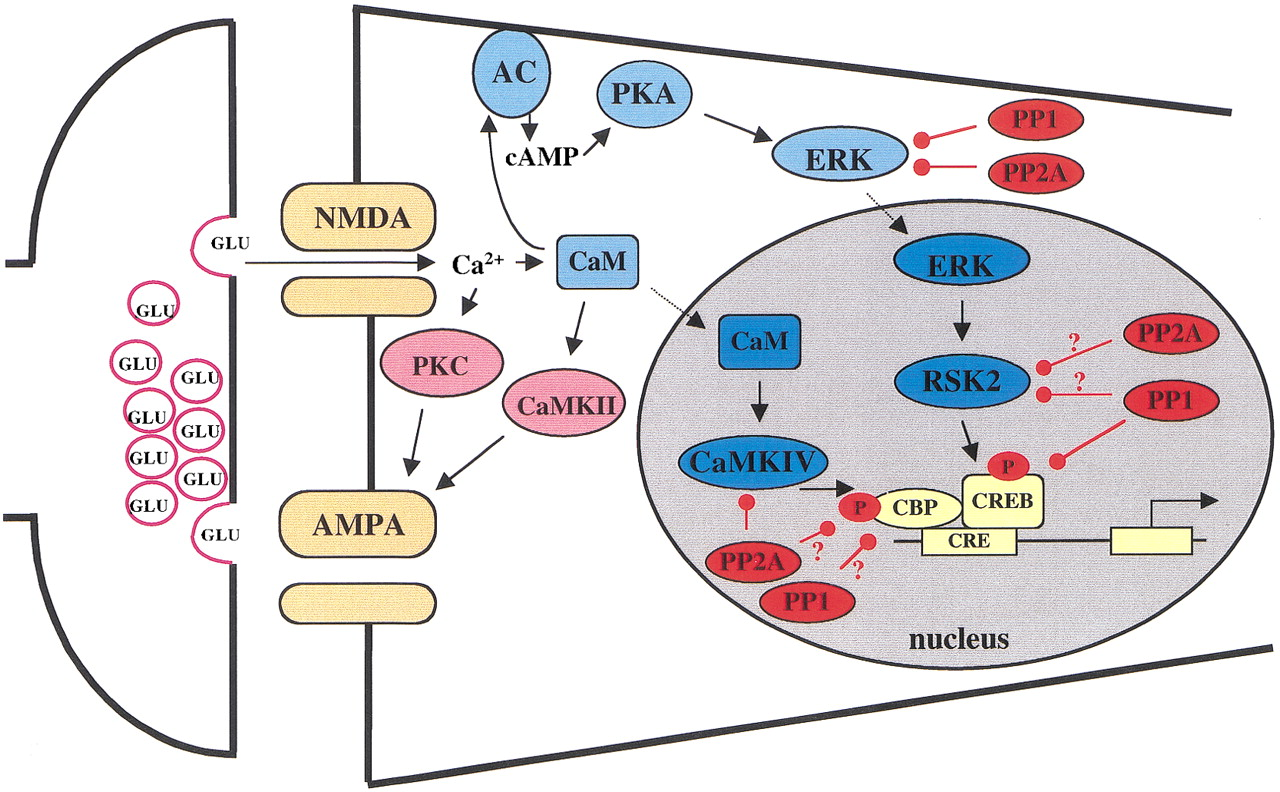
\includegraphics[width=0.95\linewidth]{plasticity-network.jpg}
  \end{center}
  %
  \citerr{Klann2002metaplasticity}
 }
 \parbox[c]{0.45\linewidth}{
  %
  \begin{center}
    \visible<2>{$W_{ij}$}
  \end{center}
  %
 }
 \end{center}
%
\end{frame}

%-------------Slide--------------------------------------------------------

\begin{frame}{Timescales of memory}
%
 \parbox[t]{0.47\linewidth}{
 Memories stored in different places for different timescales

 \citerr{Squire1995amnesia}

 \citerr{McClelland1995consolidation}
 \begin{center}
   \aligntop{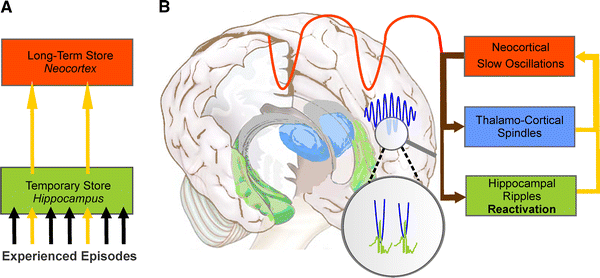
\includegraphics[width=0.9\linewidth]{sleepconsolidation.png}}
 \end{center}
 \citerr{Born2012sleep}

 Also: Cerebellar cortex \lto\ nuclei.

 \citerr{Attwell2002consolidation}

 \citerr{Cooke2004consolidation}
 }
 %
 \hspace{0.03\linewidth}
 %
 \parbox[t]{0.47\linewidth}{
 Different synapses have different molecular structures.
 \begin{center}
   \aligntop{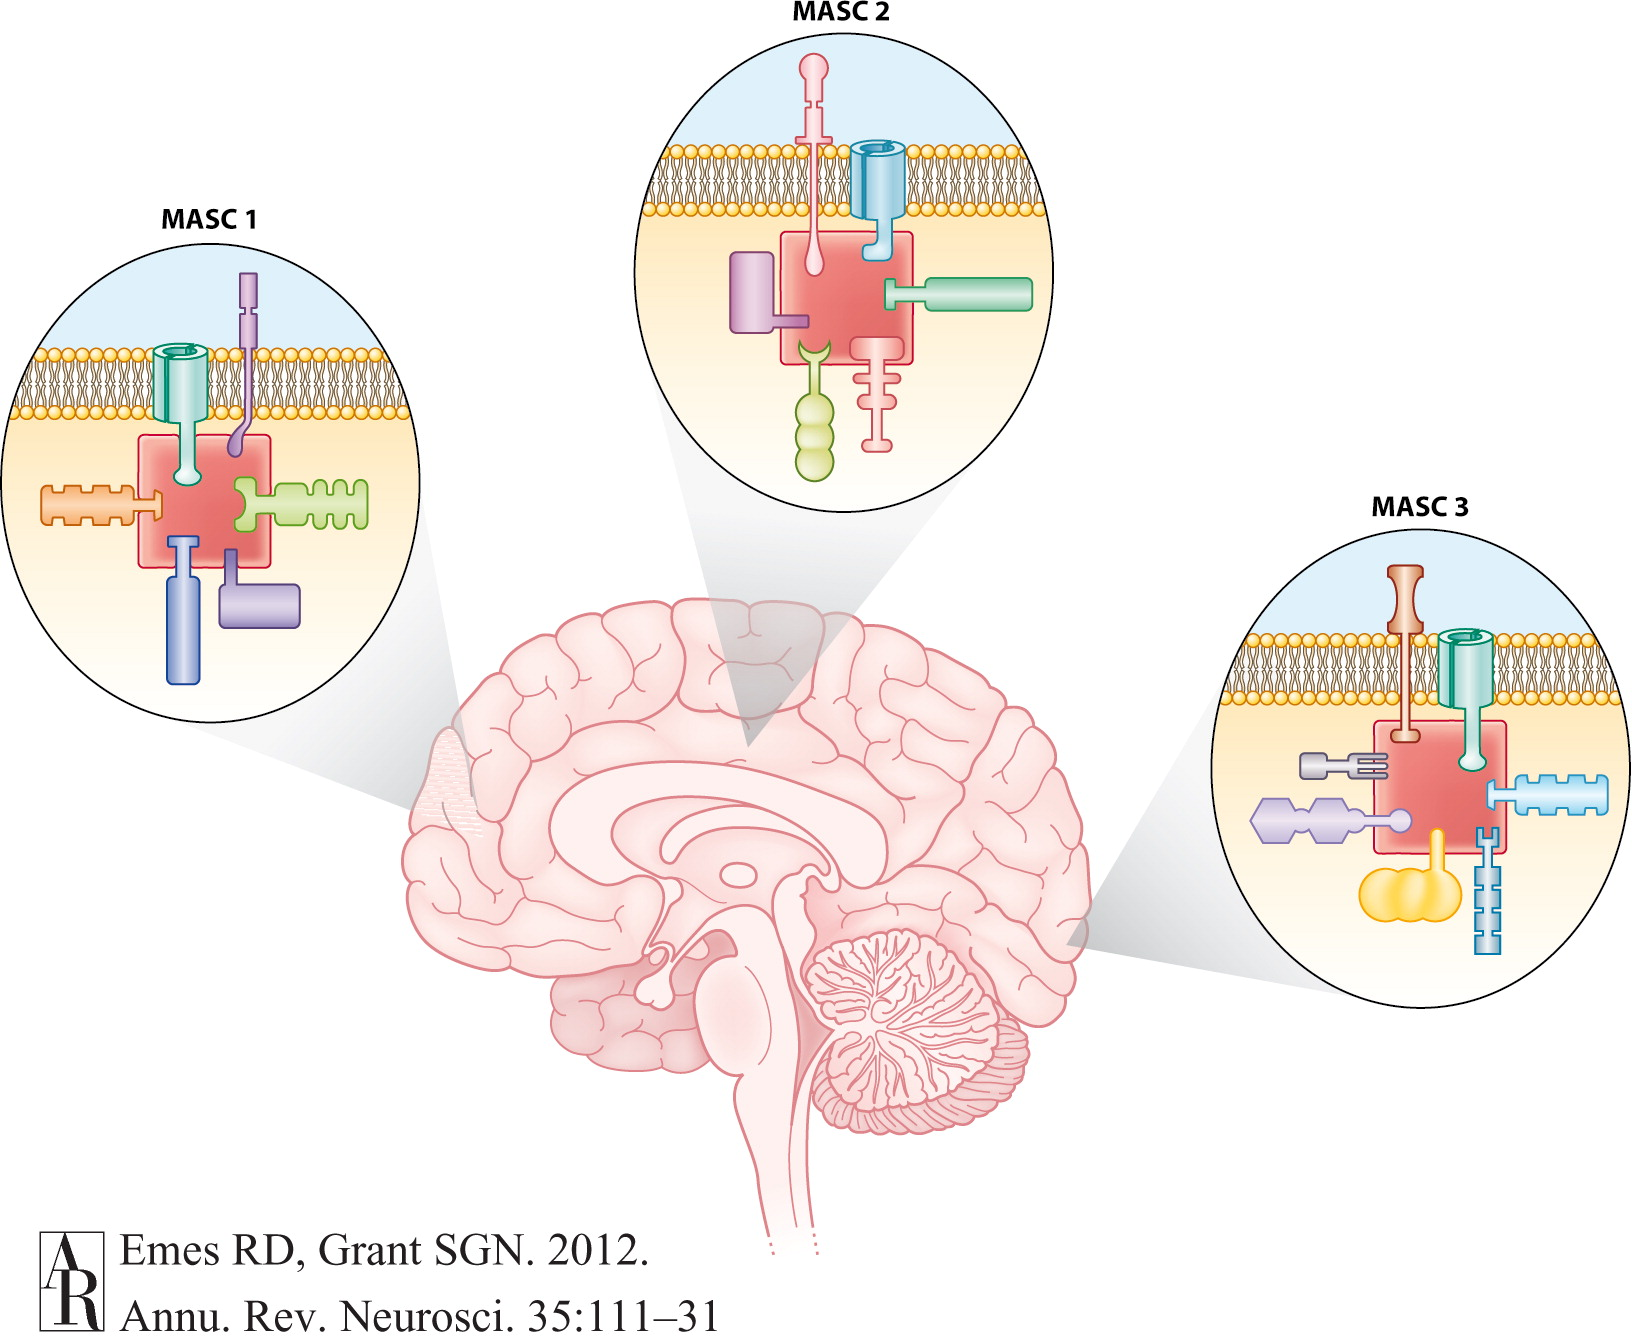
\includegraphics[width=0.8\linewidth]{Emes2012.jpeg}}
 \end{center}
 \citerr{Emes2012synapserev}
 }
 %
%
\end{frame}

%-------------Slide--------------------------------------------------------

\begin{frame}{Storage capacity of synaptic memory}
%
  A classical perceptron has a capacity $\propto N$, (\# synapses).

\vp\parbox[t]{0.59\linewidth}{%
  Requires synapses' dynamic range also $\propto N$.

 \vp With discrete, finite synapses:\\
 \hp $\implies$ new memories overwrite old,\\
 \hp $\implies$ stability-plasticity dilemma.
 %
 }
 %
 \parbox[t]{0.4\linewidth}{
   %\begin{flushright}
    \hfill\aligntop{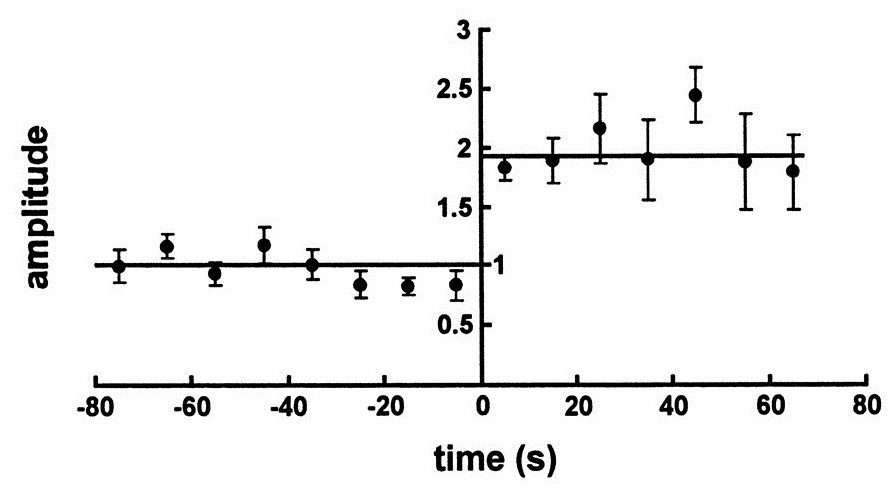
\includegraphics[width=0.9\linewidth]{Petersen1998.jpg}}
   %\end{flushright}
 }
 \\
    \citerr{Petersen1998allornone,O'Connor2005switch}

 \vp When we store new memories rapidly, memory capacity  $\sim\CO(\log N)$.
 \\ \citerr{amit1992constraints,amit1994learning}
 %
 \note[item]{or sparse $\sim \log N / N$}
%
\end{frame}


%-------------Slide--------------------------------------------------------


\begin{frame}{Recognition memory}
%
 Synapses given a sequence of patterns (pot \& dep) to store

 %\vp
 \begin{center}
 \only<1>{\aligntop{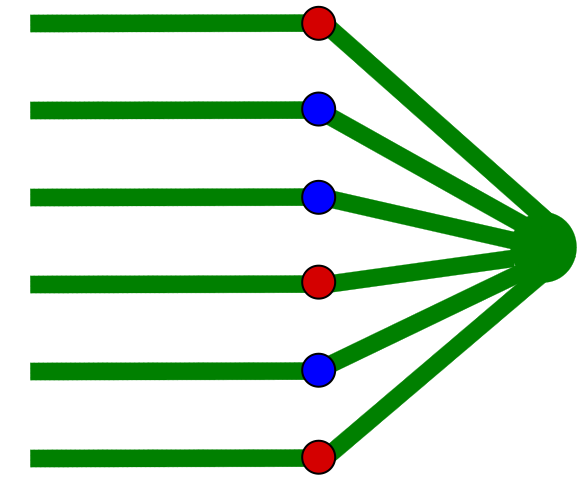
\includegraphics[width=0.275\linewidth]{perceptron1.svg}}}%
 \only<2>{\aligntop{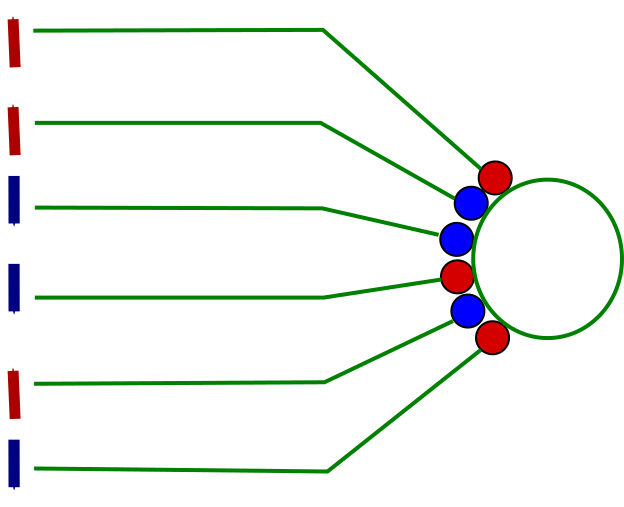
\includegraphics[width=0.275\linewidth]{perceptron2.svg}}}%
 \only<3>{\aligntop{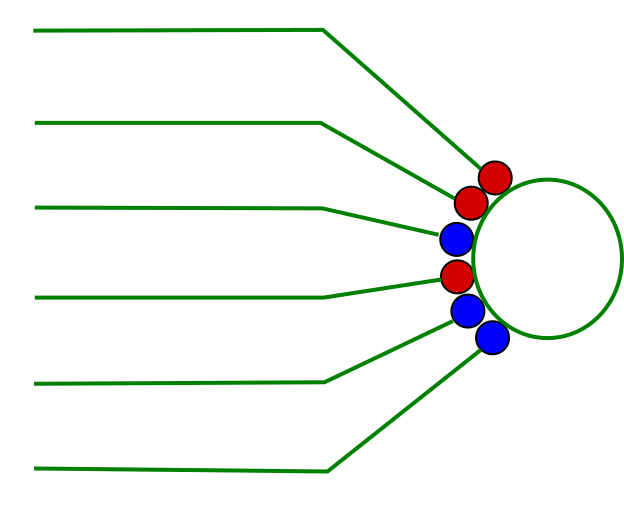
\includegraphics[width=0.275\linewidth]{perceptron3.svg}}}%
 \only<4>{\aligntop{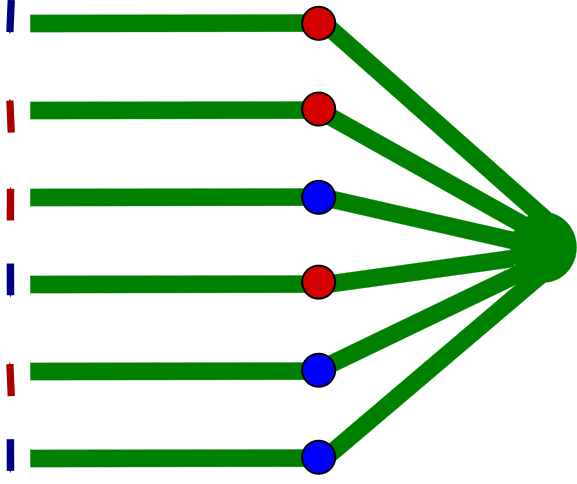
\includegraphics[width=0.275\linewidth]{perceptron4.svg}}}%
 \only<5>{\aligntop{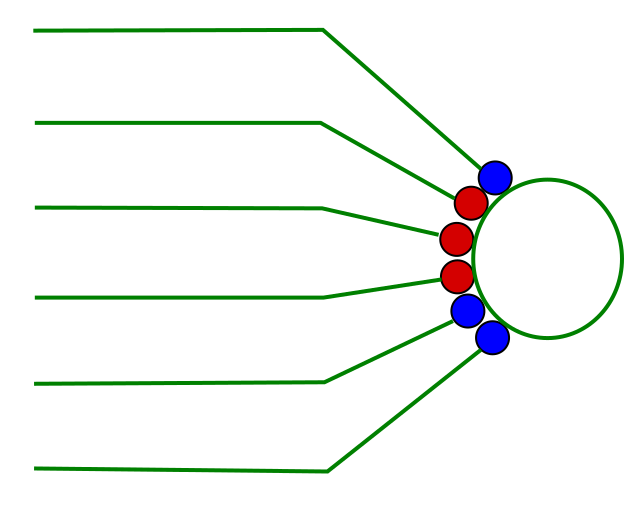
\includegraphics[width=0.275\linewidth]{perceptron5.svg}}}%
 \only<6>{\aligntop{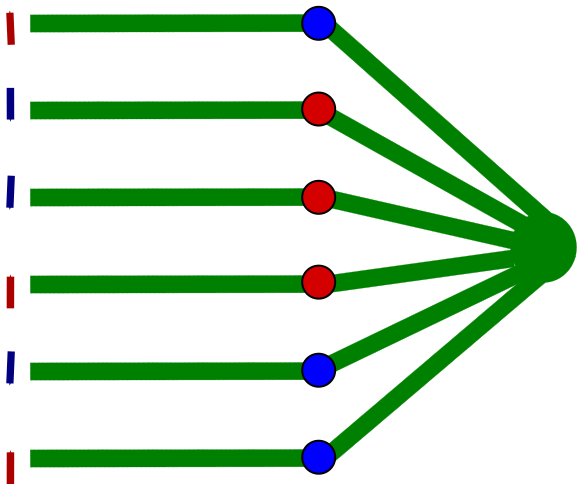
\includegraphics[width=0.275\linewidth]{perceptron6.svg}}}%
 \only<7>{\aligntop{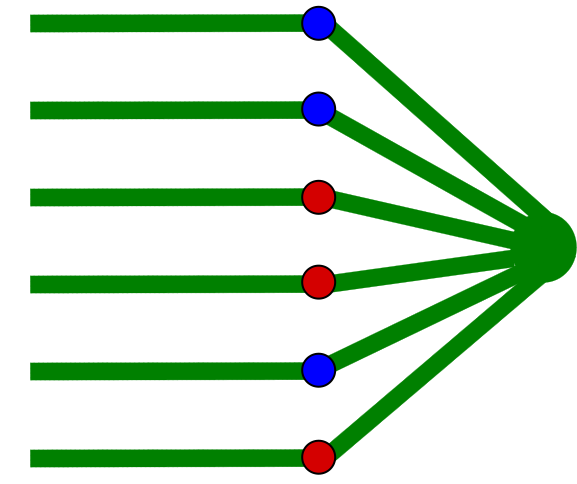
\includegraphics[width=0.275\linewidth]{perceptron7.svg}}}%
 \only<8-9>{\aligntop{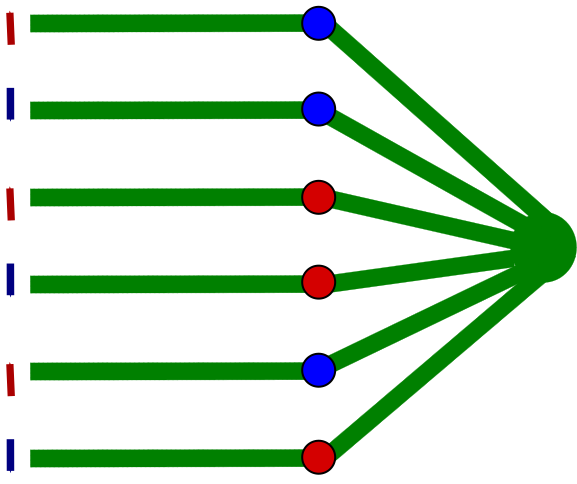
\includegraphics[width=0.275\linewidth]{perceptron8.svg}}}%
 \end{center}

 \visible<8-9>{Later: presented with a pattern.
 Has it been seen before?
%

 \vp Compare $\synid \cdot \syn(t)$ to threshold.
 \citerr{Sommer1998retrieval}}
 %
 \visible<9>{%
 %
 \begin{equation*}
     \snr(t) = \frac{ \av{\synid\cdt\syn(t)} - \av{\synid\cdt\syn(\infty)} }{ \sqrt{\var(\synid\cdt\syn(\infty))}},
     \qquad
     \snrb(\tau) = \intd{\tau} \frac{\e^{-t/\tau}}{\tau} \snr(t).
 \end{equation*}
}
%
\end{frame}

%%-------------Slide--------------------------------------------------------
%
%\begin{frame}{Quantifying memory quality}
%%
%% Have we seen pattern before?
% Test if $\synid \cdot \syn(t) \gtrless \theta$?
%
%% $\synid \cdot \syn(\infty) \sim$  null distribution
%% $\implies$ ROC curve:
%
% \vp
% %
% %
% \begin{equation*}
%   \begin{aligned}
%%   \operatorname{TPR} &= \Phi \prn{ \frac{ \snr(t) +\Phi\inv(\operatorname{FPR}) }{ \operatorname{NNR}(t) } }, \\[0.5cm]
%   %\quad\text{where } \quad
%     %\Phi(x) &= \int_{-\infty}^x \frac{ \e^{-\frac{z^2}{2}} }{ \sqrt{2\pi} }\, \dr z, \\
%     \snr(t) &= \frac{ \av{\synid\cdt\syn(t)} - \av{\synid\cdt\syn(\infty)} }{ \sqrt{\var(\synid\cdt\syn(\infty))}}, \\[1cm]
%     \snrb(\tau) &= \intd{\tau} \frac{\e^{-t/\tau}}{\tau} \snr(t).
%%     \\[1cm]
%%    \color{darkgrey} \operatorname{NNR}(t) &= \color{darkgrey} \sqrt{\frac{ \var(\synid\cdt\syn(t)) }{ \var(\synid\cdt\syn(\infty)) }}.
%   \end{aligned}
% \end{equation*}
%
%
%%
%\end{frame}
%
%-------------Slide--------------------------------------------------------

\begin{frame}{Models of complex synaptic dynamics}
%
%  There are $N$ identical synapses with $M$ internal functional states.
\visible<2->{
\parbox[c]{0.82\linewidth}{%
  \begin{itemize}
    \item Internal functional state of synapse \lto\ synaptic weight.
    \item Candidate plasticity events \lto\ transitions between states
  \end{itemize}
}\hfill
\alignmid{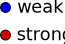
\includegraphics[width=0.13\linewidth]{state_key.svg}}
}

  %
  \vp
%  \begin{overlayarea}{0.7\linewidth}{0.3\linewidth}
%    \only<1>{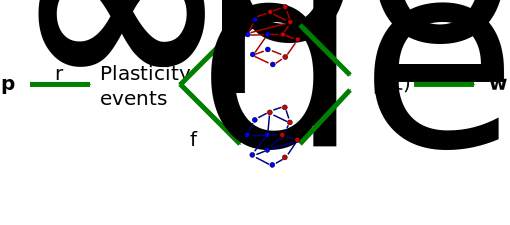
\includegraphics[width=0.99\linewidth]{synapse_model_1.svg}}%
%    \only<2>{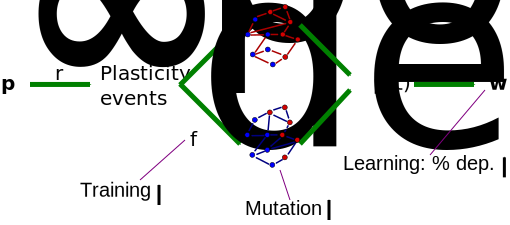
\includegraphics[width=0.99\linewidth]{synapse_model_2.svg}}
%  \end{overlayarea}
%
\begin{overlayarea}{0.95\linewidth}{0.4\textheight}
  \begin{center}
%\aligntop{\movie[width=200px,height=92px,showcontrols=true,loop]{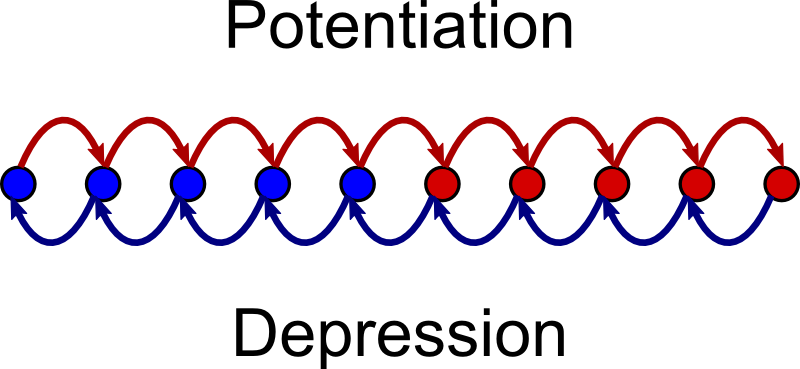
\includegraphics[width=200px,height=92px]{Vids/plast_00.png}}{plast.avi}}
    \only<1>{\aligntop{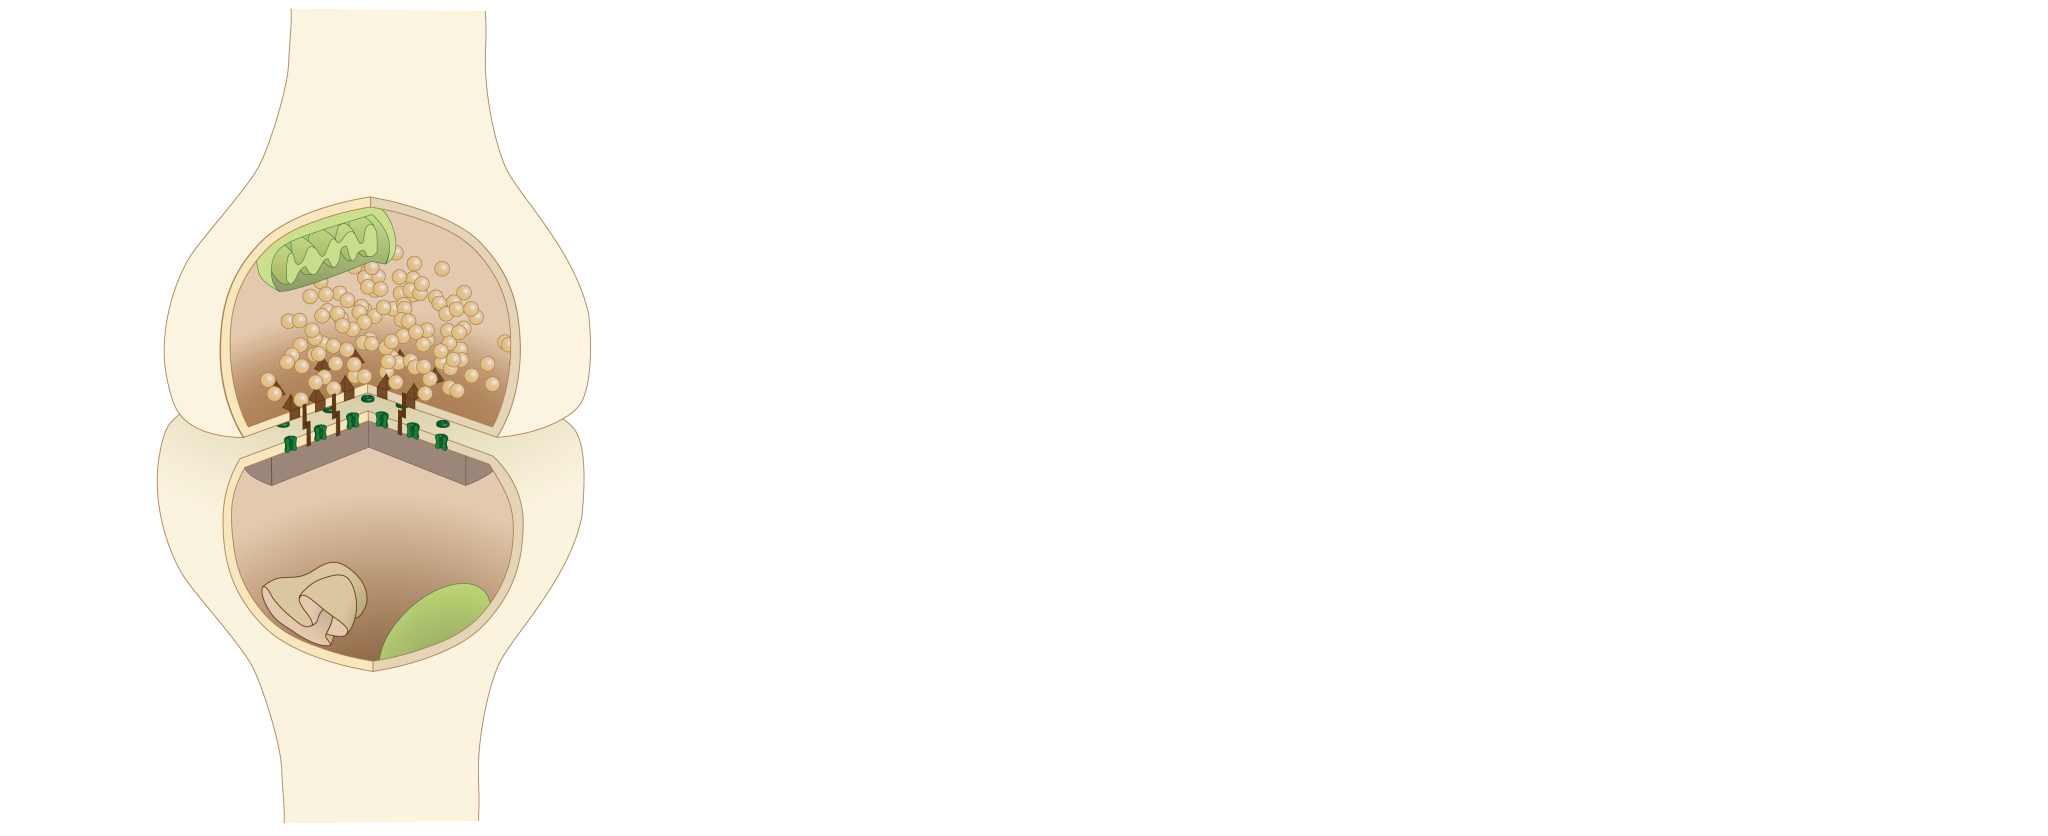
\includegraphics[width=0.7\linewidth]{serial_internal_1.svg}}}%
    \only<2>{\aligntop{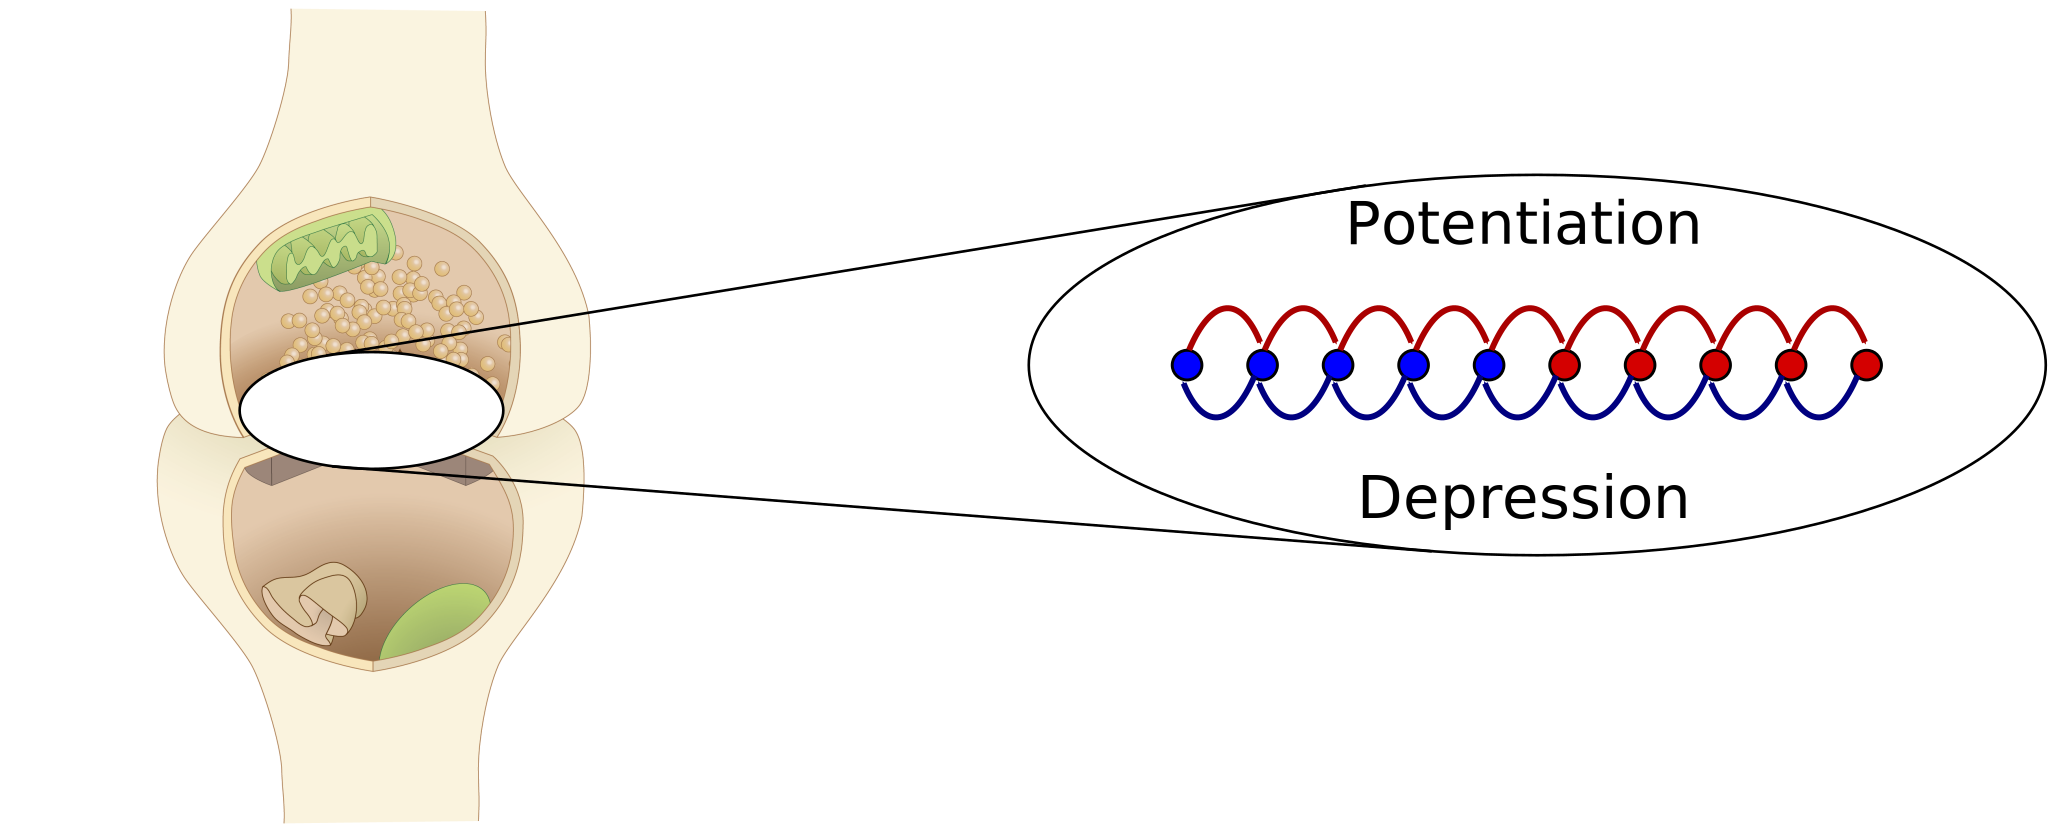
\includegraphics[width=0.7\linewidth]{serial_internal.svg}}}%
    \only<3->{\vp}
    \only<3>{\aligntop{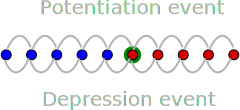
\includegraphics[width=0.5\linewidth]{Animation/serial_anim_01.svg}}}%
    \only<4>{\aligntop{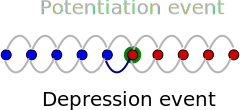
\includegraphics[width=0.5\linewidth]{Animation/serial_anim_02.svg}}}%
    \only<5>{\aligntop{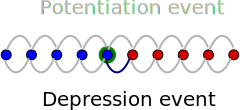
\includegraphics[width=0.5\linewidth]{Animation/serial_anim_03.svg}}}%
    \only<6>{\aligntop{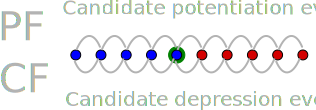
\includegraphics[width=0.5\linewidth]{Animation/serial_anim_04.svg}}}%
    \only<7>{\aligntop{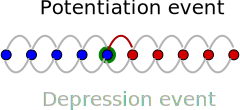
\includegraphics[width=0.5\linewidth]{Animation/serial_anim_05.svg}}}%
    \only<8>{\aligntop{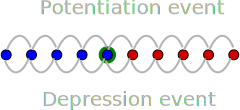
\includegraphics[width=0.5\linewidth]{Animation/serial_anim_06.svg}}}%
%    \only<9>{\aligntop{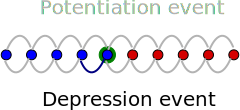
\includegraphics[width=0.5\linewidth]{Animation/serial_anim_07.svg}}}%
%    \only<10>{\aligntop{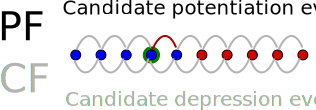
\includegraphics[width=0.5\linewidth]{Animation/serial_anim_08.svg}}}%
%    \only<11>{\aligntop{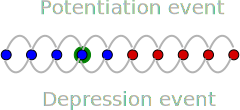
\includegraphics[width=0.5\linewidth]{Animation/serial_anim_09.svg}}}%
%    \only<12>{\aligntop{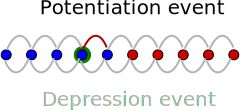
\includegraphics[width=0.5\linewidth]{Animation/serial_anim_10.svg}}}%
%    \only<13>{\aligntop{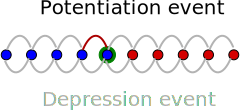
\includegraphics[width=0.5\linewidth]{Animation/serial_anim_11.svg}}}%
%    \only<14>{\aligntop{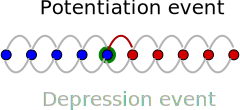
\includegraphics[width=0.5\linewidth]{Animation/serial_anim_12.svg}}}%
%    \only<15>{\aligntop{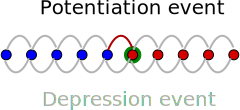
\includegraphics[width=0.5\linewidth]{Animation/serial_anim_13.svg}}}%
%    \only<16>{\aligntop{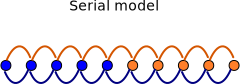
\includegraphics[width=0.5\linewidth]{Animation/serial.svg}}}%
%    \only<5>{\aligntop{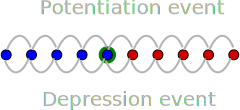
\includegraphics[width=0.5\linewidth]{Animation/serial_anim_06.svg}}}%
%    \only<6>{\aligntop{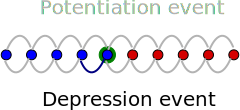
\includegraphics[width=0.5\linewidth]{Animation/serial_anim_07.svg}}}%
%    \only<7>{\aligntop{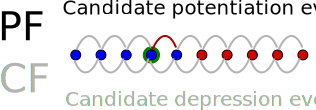
\includegraphics[width=0.5\linewidth]{Animation/serial_anim_08.svg}}}%
%    \only<8>{\aligntop{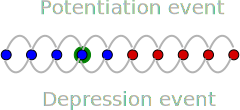
\includegraphics[width=0.5\linewidth]{Animation/serial_anim_09.svg}}}%
%    \only<9>{\aligntop{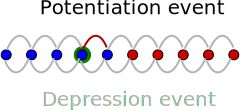
\includegraphics[width=0.5\linewidth]{Animation/serial_anim_10.svg}}}%
%    \only<10>{\aligntop{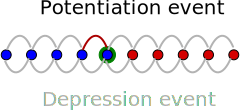
\includegraphics[width=0.5\linewidth]{Animation/serial_anim_11.svg}}}%
%    \only<11>{\aligntop{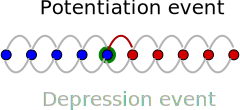
\includegraphics[width=0.5\linewidth]{Animation/serial_anim_12.svg}}}%
%    \only<12>{\aligntop{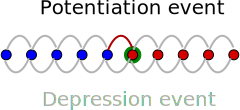
\includegraphics[width=0.5\linewidth]{Animation/serial_anim_13.svg}}}%
    \only<9>{\aligntop{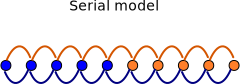
\includegraphics[width=0.5\linewidth]{Animation/serial.svg}}}%
    %
%    \hspace{0.05\linewidth}\parbox[t]{0.45\linewidth}{\raggedright
%    \visible<15>{
%    Mutation: transition probabilities \\ \vp
%    Training: rates of pot/dep events \\ \vp
%    Learning: synaptic weight}}
  \end{center}
\end{overlayarea}

%  \onslide<2>{\hfill
%  \parbox[t]{0.3\linewidth}{PF+\cancel{CF} \lto\ LTP, \\
%              PF+CF \lto\ LTD.}
%  \parbox[t]{0.27\linewidth}{Lower threshold\\ for LTD}
%  \parbox[t]{0.27\linewidth}{VOR gain increase}}
\vp
\begin{overlayarea}{0.95\linewidth}{0.3\textheight}
  \only<2>{States: \parbox[t]{0.85\linewidth}{\#AMPAR, \#NMDAR, NMDAR subunit composition, \\
   CaMK II autophosphorylation, activating PKC, p38 MAPK,...}

  \vp\footnotesize\citerr{Fusi2005cascade,Fusi2007multistate,Barrett2008discrete}}%
  %\\\citerr{Smith2006savings,Lahiri2013synapse}}%

%  \only<8->{Metaplasticity: \parbox[t]{0.7\linewidth}{%
%     change propensity for plasticity \\
%     (independent of change in synaptic weight).}}
\end{overlayarea}

  %
  \note[item]{complex synapse: not just synaptic weight. dynamical system}
  \note[item]{important for memory with bounded synapses}
  \note[item]{nodes \lto\ states}
  \note[item]{color \lto\ sttrength}
  \note[item]{arrows \lto\ plasticity}
%  \note[item]{stoch process has steady state distribution.}
%  \note[item]{Prior activity puts it in this state. row vec.}
  \note[item]{plasticity events at rate r. indep at each synapse.}
  \note[item]{fraction pot/dep}
  \note[item]{Readout: synaptic weight vec when in each state.}
    \note[item]{Mutation: lower threshold \lto\ increase transition probs}
    \note[item]{Training: Changes statistics of LTP/LTD. Only parameters we have. Don't care about $r$.}
    \note[item]{Learning: Only output we have. Don't keep track of synaptic identity.}
%    \note<2>[item]{Same PF+CF input \lto\ same $r,f\pot,f\dep$ in each case.}
%    \note<2>[item]{Input to Pk, some linear combination of $\w$'s. }
% At $t=0$, the memory is created by $\M\potdep$ with probability $f\potdep$.
% \note[item]{for this one, we keep track of pot/dep, look for inc/dec of $\w$}
%
% \vp Forgetting caused by subsequent memories, evolving as
%
%  \begin{equation*}
%  \begin{aligned}
%    \diff{\pr(t)}{t} &= r\pr(t)\frg,
%    &\qquad
%    \frg &= f\pot\M\pot+f\dep\M\dep-\I,\\&&
%    \eq\frg &=0.
%  \end{aligned}
%  \end{equation*}
%%
%  \note[item]{Memory at $t=0$, keep track of pot/dep}
%  \note[item]{subsequent: average over pot/dep}
% \note[item]{$\frg$ is forgetting matrix, $\I=$identity, don't keep track of pot/dep}
% Eventually, this will settle into the equilibrium distribution:
% %
% %
% \note[item]{In equilibrium prior to memory creation}
%
\end{frame}

%%-------------Slide--------------------------------------------------------
%
%\begin{frame}{Upper bounds on measures of memory}
%%
% Initial SNR:
% %
% \begin{equation*}
%   \snr(0) = \snrb(0) \leq \sqrt{N}.
% \end{equation*}
% %
% %
% \begin{center}
%   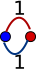
\includegraphics[height=0.1\linewidth]{binary_det.svg}
% \end{center}
% %
% Area under curve:
% %
% \begin{equation*}
%   \area = \intd[_0^\infty]{t} \snr(t) = \lim_{\tau\ra\infty} \tau \, \snrb(\tau) \leq \sqrt{N}(M-1)/r.
% \end{equation*}
% %
% %
% \begin{center}
%   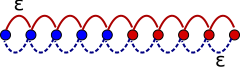
\includegraphics[height=0.1\linewidth]{multistate_sticky.svg}
% \end{center}
% %
% \citerr{Lahiri2013synapse}
%%
%\end{frame}
%
%-------------Slide--------------------------------------------------------

\begin{frame}{Proven envelope: memory frontier}
%
 \visible<2->{Upper bound on memory curve at \emph{any} timescale.}

 \vp
% \begin{center}
 \parbox[c]{0.67\linewidth}{
   \only<1>{\aligntop{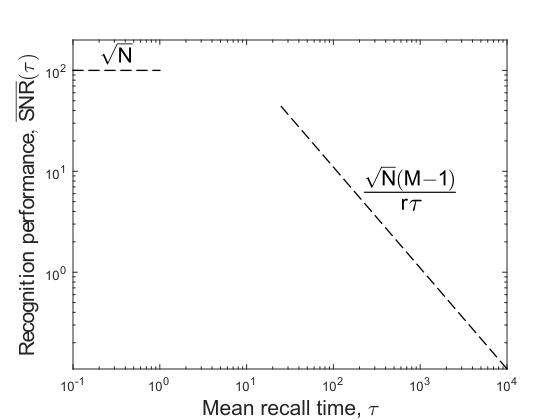
\includegraphics[width=0.95\linewidth]{RunAveProvenNum2.svg}}}%
   \only<2>{\aligntop{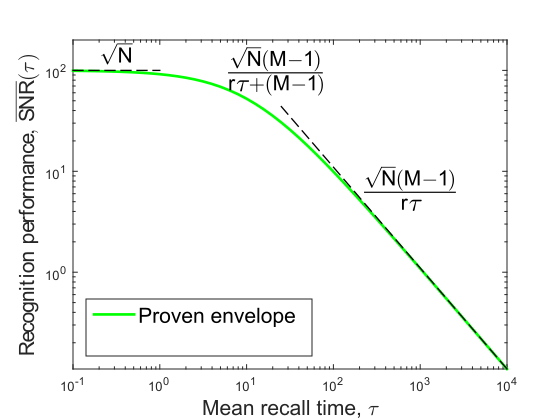
\includegraphics[width=0.95\linewidth]{RunAveProvenNum1.svg}}}%
   \only<3>{\aligntop{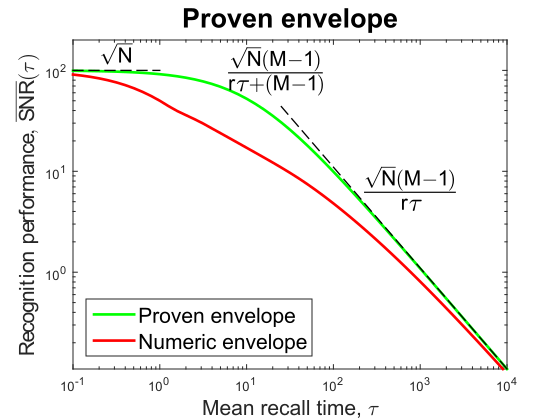
\includegraphics[width=0.95\linewidth]{RunAveProvenNum.svg}}}%
   \note[item]{Best we've found, by numerical opt and hand chosen models.}
% \note[item]{Models on next slide}
 }
% \end{center}
% \hspace{0.01\linewidth}
 %
 \visible<3>{
 \parbox[c]{0.3\linewidth}{
   Serial topology:
   %
   \begin{center}
  %   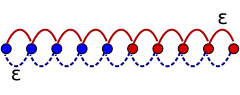
\includegraphics[width=6cm]{multistate_shorten.svg}
     \includegraphics[width=0.99\linewidth]{multistate.svg}
   \end{center}
   %
 }}
 \note[item]{Gap $\sim\CO(\sqrt{N})$.}
 \note[item]{Area bound active at early times $\implies$ need more constraints.}
%
\end{frame}


%-------------Slide--------------------------------------------------------

%\begin{frame}{Models that maximise memory for one timescale}
%%
% %
% \begin{center}
%   \only<1>{\aligntop{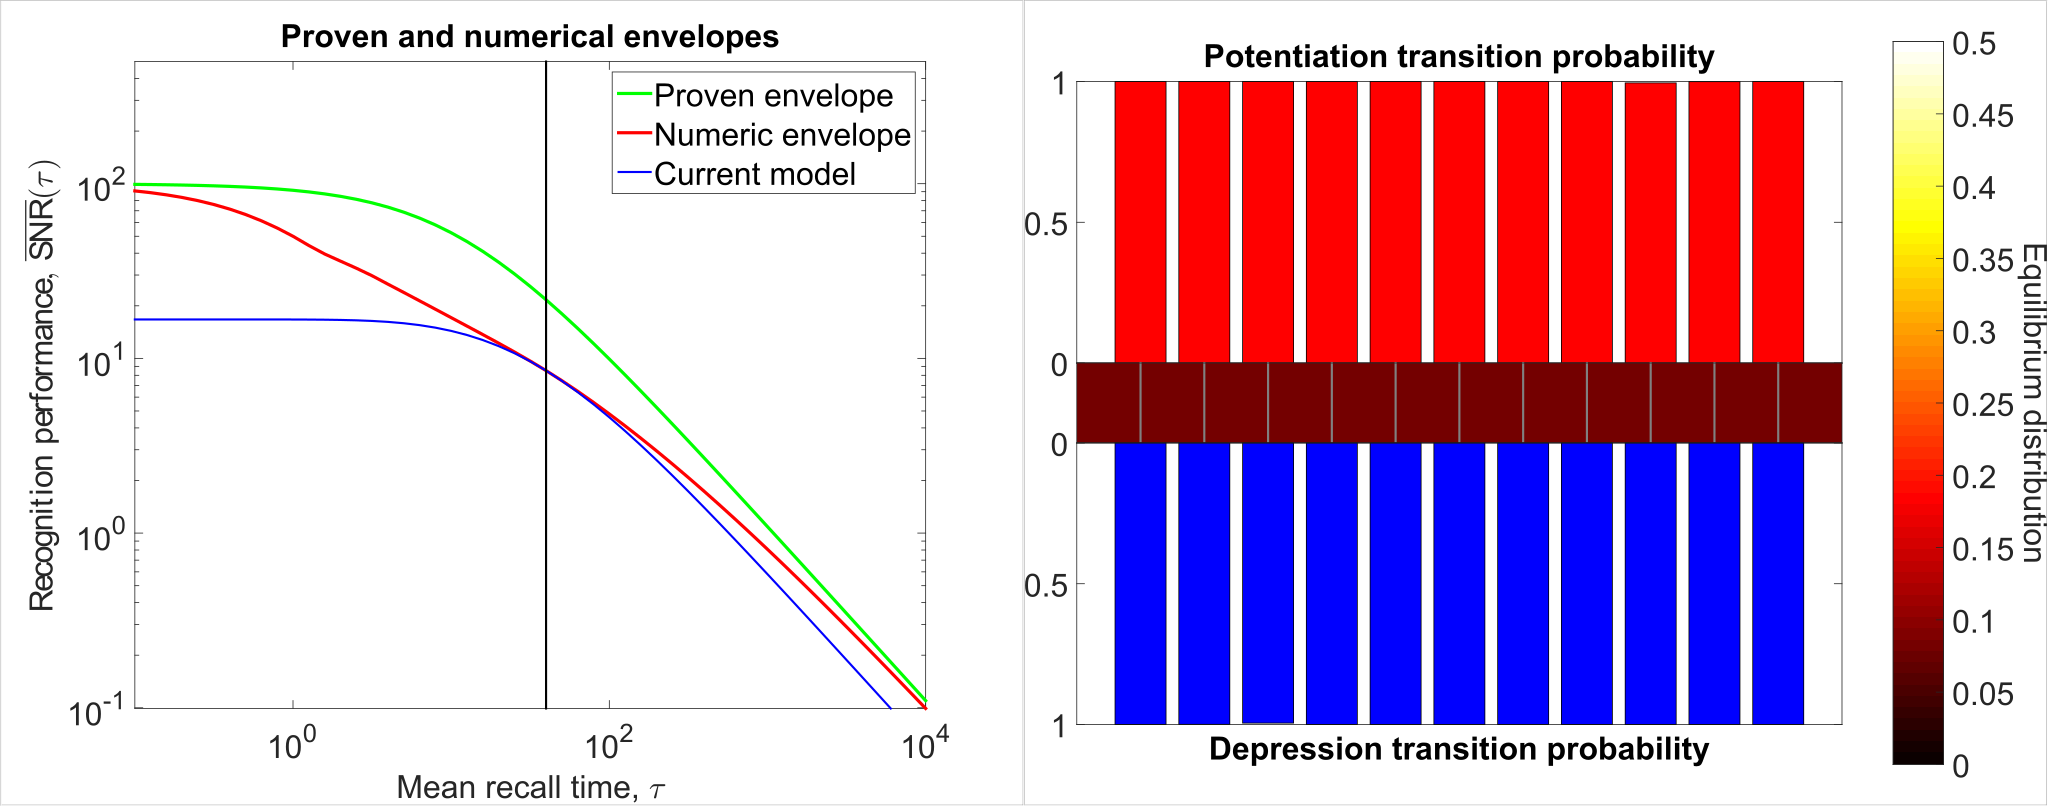
\includegraphics[width=0.9\linewidth]{Animation/Lenv27.svg}}}%
%   %\only<2>{\aligntop{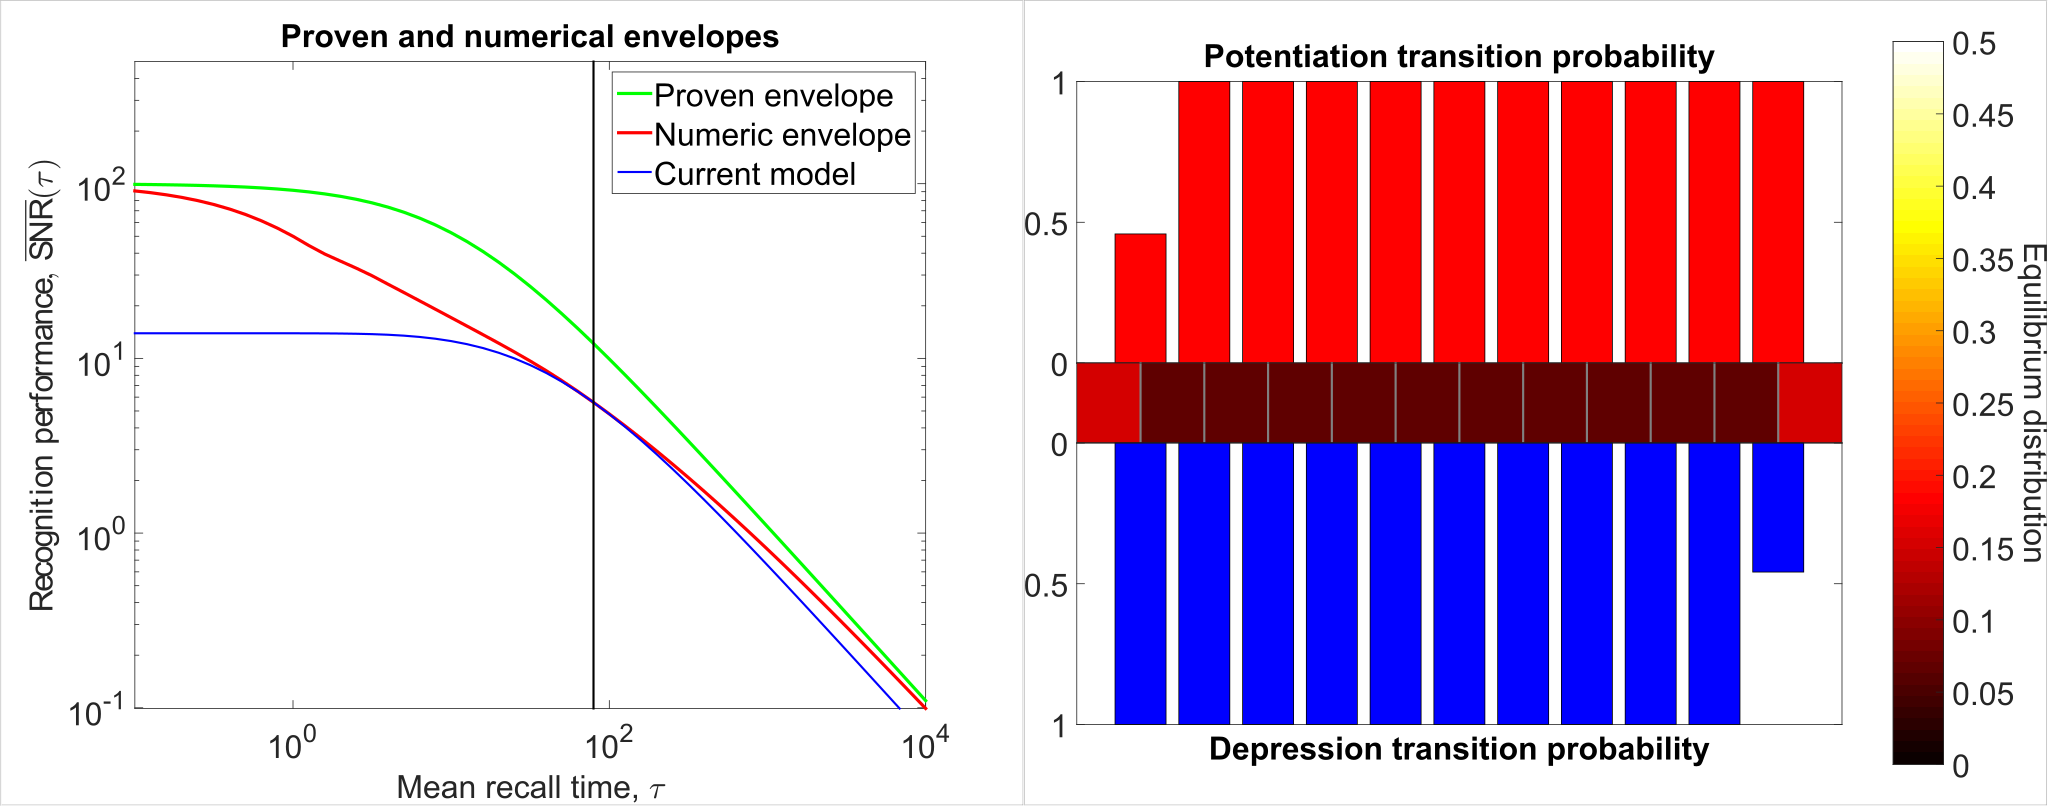
\includegraphics[width=0.9\linewidth]{Animation/Lenv30.svg}}}%
%   \only<2>{\aligntop{\includegraphics[width=0.9\linewidth]{Animation/Lenv34.svg}}}%
%   %\only<2>{\aligntop{\includegraphics[width=0.9\linewidth]{Animation/Lenv42.svg}}}%
%   \only<3>{\aligntop{\includegraphics[width=0.9\linewidth]{Animation/Lenv47.svg}}}%
%   %\only<6>{\aligntop{\includegraphics[width=0.9\linewidth]{Animation/Lenv51.svg}}}%
%   %
%   \only<4>{\aligntop{\includegraphics[width=0.9\linewidth]{Animation/Lenv27.svg}}}%
%   %\only<8>{\aligntop{\includegraphics[width=0.9\linewidth]{Animation/Lenv24.svg}}}%
%   %\only<9>{\aligntop{\includegraphics[width=0.9\linewidth]{Animation/Lenv21.svg}}}%
%   \only<5>{\aligntop{\includegraphics[width=0.9\linewidth]{Animation/Lenv20.svg}}}%
%   %\only<11>{\aligntop{\includegraphics[width=0.9\linewidth]{Animation/Lenv19.svg}}}%
%   %\only<12>{\aligntop{\includegraphics[width=0.9\linewidth]{Animation/Lenv17.svg}}}%
%   \only<6>{\aligntop{\includegraphics[width=0.9\linewidth]{Animation/Lenv16.svg}}}%
%   %\only<14>{\aligntop{\includegraphics[width=0.9\linewidth]{Animation/Lenv14.svg}}}%
%   %\only<15>{\aligntop{\includegraphics[width=0.9\linewidth]{Animation/Lenv12.svg}}}%
%   \only<7>{\aligntop{\includegraphics[width=0.9\linewidth]{Animation/Lenv06.svg}}}%
%   %\only<17>{\aligntop{\includegraphics[width=0.9\linewidth]{Animation/Lenv01.svg}}}%
% \end{center}
%%
%%
%\end{frame}
%
%
%-------------Slide--------------------------------------------------------
%
%\begin{frame}{Heuristic envelope}
%%
% %
% \begin{center}
%   \includegraphics[width=0.88\linewidth]{LenvAnalytic.svg}
% \end{center}
%%
%%
%\end{frame}
%
%-------------Slide--------------------------------------------------------

\begin{frame}{Synaptic structures for different timescales of memory}
%
% Real synapses limited by molecular building blocks. \\
% Evolution had larger set of priorities.
%
% \vp What can we conclude?

 \begin{center}
 \begin{tabular}{ccccc}
   % after \\: \hline or \cline{col1-col2} \cline{col3-col4} ...
   Short timescales & $\longrightarrow$ & Intermediate timescales & $\longrightarrow$ & Long timescales \\[0.5cm]
   \alignmid{\includegraphics[height=0.065\linewidth]{binary_det.svg}} & $\longrightarrow$ & \alignmid{\includegraphics[height=0.065\linewidth]{multistate_uni.svg}} & $\longrightarrow$ & \alignmid{\includegraphics[height=0.065\linewidth]{multistate_sticky.svg}} \\[0.5cm]
   \visible<2->{short \& wide} & \visible<2->{$\longrightarrow$} & \visible<2->{long \& thin} &  &  \\[0.5cm]
    & & \visible<3->{strong transitions} & \visible<3->{$\longrightarrow$} & \visible<3->{weak transitions} \\
 \end{tabular}
 \end{center}
%
\end{frame}


%-------------Slide--------------------------------------------------------

\begin{frame}{Proposed Experimental design}
%
 Subject a synapse to a sequence of candidate plasticity events.

 Observe the changes in synaptic efficacy.

 \begin{center}
     \only<1>{\aligntop{\includegraphics[width=0.1\linewidth]{single_synapse_depstrong.svg}}}%
     \only<2>{\aligntop{\includegraphics[width=0.1\linewidth]{single_synapse_depweak.svg}}}%
     \only<3>{\aligntop{\includegraphics[width=0.1\linewidth]{single_synapse_potweak.svg}}}%
     \only<4>{\aligntop{\includegraphics[width=0.1\linewidth]{single_synapse_depweak.svg}}}%
     \only<5>{\aligntop{\includegraphics[width=0.1\linewidth]{single_synapse_potstrong.svg}}}%
     \only<6->{\aligntop{\includegraphics[width=0.1\linewidth]{single_synapse_potstrong.svg}}}%
 \end{center}

 \visible<7->{\textbf{EM algorithms:}

   Sequence of hidden states $\ra$ estimate transition probabilities \\
   Transition probabilities $\ra$ estimate sequence of hidden states

   \citerr{Baum1970baumwelch,rabiner1993speechrec,Dempster2007EM}

% \vp \textbf{Spectral algorithms:}
%
% Compute $P(w_1), P(w_1,w_2), P(w_1,w_2,w_3),\ldots$  \hp
% \parbox[t]{0.3\linewidth}{
%   from data, \\
%   from model.
% }
%
% \citerr{Hsu2008hmmspec}
 }
%
\end{frame}

%-------------Slide--------------------------------------------------------

\begin{frame}{Simulated experiment}
%
 %
 \begin{center}
%   \only<1>{\aligntop{\includegraphics[width=0.97\linewidth]{Animation/FitVid00.svg}}}%
%   \only<2>{\aligntop{\includegraphics[width=0.97\linewidth]{Animation/FitVid104.svg}}}%
%   \only<3>{\aligntop{\includegraphics[width=0.97\linewidth]{Animation/FitVid208.svg}}}%
%   \only<4>{\aligntop{\includegraphics[width=0.97\linewidth]{Animation/FitVid312.svg}}}%
%   \only<5>{\aligntop{\includegraphics[width=0.97\linewidth]{Animation/FitVid416.svg}}}%
%   \only<6>{\aligntop{\includegraphics[width=0.97\linewidth]{Animation/FitVid520.svg}}}%
%   \only<7>{\aligntop{\includegraphics[width=0.97\linewidth]{Animation/FitVid624.svg}}}%
%   \only<8>{\aligntop{\includegraphics[width=0.97\linewidth]{Animation/FitVid728.svg}}}%
%   \only<9>{\aligntop{\includegraphics[width=0.97\linewidth]{Animation/FitVid832.svg}}}%
%   \only<10>{\aligntop{\includegraphics[width=0.97\linewidth]{Animation/FitVid939.svg}}}%
   \only<1>{\aligntop{\includegraphics[width=0.97\linewidth]{Animation/FitVid00.svg}}}%
   \only<2>{\aligntop{\includegraphics[width=0.97\linewidth]{Animation/FitVid104.svg}}}%
%   \only<3>{\aligntop{\includegraphics[width=0.97\linewidth]{Animation/FitVid208.svg}}}%
   \only<3>{\aligntop{\includegraphics[width=0.97\linewidth]{Animation/FitVid312.svg}}}%
%   \only<5>{\aligntop{\includegraphics[width=0.97\linewidth]{Animation/FitVid416.svg}}}%
   \only<4>{\aligntop{\includegraphics[width=0.97\linewidth]{Animation/FitVid520.svg}}}%
%   \only<7>{\aligntop{\includegraphics[width=0.97\linewidth]{Animation/FitVid624.svg}}}%
%   \only<5>{\aligntop{\includegraphics[width=0.97\linewidth]{Animation/FitVid728.svg}}}%
%   \only<9>{\aligntop{\includegraphics[width=0.97\linewidth]{Animation/FitVid832.svg}}}%
   \only<5>{\aligntop{\includegraphics[width=0.97\linewidth]{Animation/FitVid939.svg}}}%
 \end{center}
 %
%
\end{frame}


%%-------------Slide--------------------------------------------------------
%
%\begin{frame}{Experimental problems}
%%
% \begin{itemize}
%   \item Need single synapses.
%   \item Need long sequences of plasticity events.
%   \item Need to control types of candidate plasticity events.
%   \item Need to measure synaptic efficacies.
% \end{itemize}
%
% \vp When we patch the postsynaptic neuron \lto\ Ca washout.
%%
%\end{frame}
%
%-------------Slide--------------------------------------------------------

\begin{frame}{Summary}
%
  \begin{itemize}
    \item We have formulated a general theory of learning and memory with complex synapses.
%    \item We can impose an order on the internal states of a synapse through the theory of first passage times.
%    \item The area under the memory curve of any model $<$ linear chain with same equilibrium distribution.
    \vp\item We find a memory envelope: a single curve that cannot be exceeded by the memory curve of \emph{any} synaptic model.
%    \vp\item Synaptic complexity ($M$ internal states) raises the memory envelope linearly in $M$ for times $> \CO(M^2)$.
    \vp\item We understood which types of synaptic structure are useful for storing memories for different timescales.
%    \item Gap between envelope and what we can achieve at early times?
%    \item Trade-off between SNR at different times?
%    \item For times $< \CO(M^2)$: conjecture that the model that reaches the envelope uses deterministic transitions $\to$ diffusive forgetting.
  \end{itemize}

%
\end{frame}





%-------------Slide--------------------------------------------------------
%
%% Press Ctrl-D to insert a new slide
%
%
%-------------Slide--------------------------------------------------------

\begin{frame}{Acknowledgements}
%
\parbox[t]{0.4\linewidth}{
 Thanks to:
 \begin{itemize}
   \item Surya Ganguli
   \item Stefano Fusi
   \item Marcus Benna
   \item David Sussillo
   \item Jascha Sohl-Dickstein
 \end{itemize}
 }
\parbox[t]{0.4\linewidth}{
 Funding:
 \begin{itemize}
   \item Swartz foundation
   \item Stanford Bio-X
   \item Genentech
 \end{itemize}
 }
 \note[item]{Last slide!}
%
\end{frame}

%-------------Slide--------------------------------------------------------
\appendix
%-------------Slide--------------------------------------------------------

\begin{frame}[allowframebreaks]{References}
%

 {\small
 \bibliographystyle{unsrt_slides}
 \bibliography{maths,neuro,markov}
 }
%
\end{frame}

%-------------Slide--------------------------------------------------------

\begin{frame}[label=fr_tech]{Technical detail: ordering states}
%
 Let $\fpt_{ij}=$ mean first passage time from state $i$ to state $j$.
 Then:
 %
 \begin{equation*}
   \eta = \sum_j \fpt_{ij} \eq_j,
 \end{equation*}
 %
 is independent of the initial state $i$
 (Kemeney's constant).\\ \citerr{kemeny1960finite}

 \vp We define:
 %
 \begin{equation*}
   \eta^+_i = \sum_{j\in\text{strong}} \fpt_{ij} \eq_j,
   \qquad
   \eta^-_i = \sum_{j\in\text{weak}} \fpt_{ij} \eq_j.
 \end{equation*}
 %
 \note[item]{Measure ``distance'' to the strong/weak states.}
 They can be used to arrange the states in an order (increasing $\eta^-$ or decreasing $\eta^+$).
 \hyperlink{fr_areaproof}{\beamerbutton{back}}
 \note[item]{sum to constant, $\implies$ two orders same}
%
\end{frame}

%-------------Slide--------------------------------------------------------

\begin{frame}{Technical detail: upper/lower triangular}
%
 With states in order:
 %
 \begin{center}
   \includegraphics[width=2cm]{triangular_right.svg}
   \hp \hp \hp
   \includegraphics[width=2cm]{triangular_left.svg}
 \end{center}
 %
 \note[item]{pot \& dep with same initial \& final state}
 Endpoint: potentiation goes right, depression goes left.
 \note[item]{pot/dep matrices are upper/lower triangular.}
 \note[item]{one other pert. too technical, even for bonus slide!}

 \hyperlink{fr_areaproof}{\beamerbutton{back}}
%
\end{frame}


%-----End----------------------------------------------------------------

\end{document}
